\begin{frame}
  \frametitle{Rad van Fortuin}
  \begin{center}
    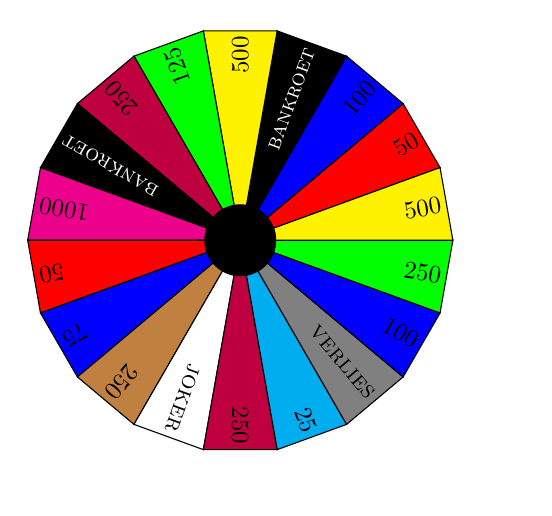
\begin{tikzpicture}[scale=.9,transform shape]
      \path[use as bounding box] (-3,-3.5) rectangle (4,3);

      \foreach[count=\i] \text/\c in {50/red,100/blue,{\color{white}\sc\small bankroet}/black,500/yellow,125/green,250/purple,{\color{white}\sc\small bankroet}/black,1000/magenta,50/red,75/blue,250/brown,{\sc joker}/white,250/purple,25/cyan,{\sc verlies}/gray,100/blue,250/green,500/yellow} {
        \pgfmathparse{20}\let\deltaangle\pgfmathresult
        \pgfmathparse{\i * \deltaangle}\let\startangle\pgfmathresult
        \pgfmathparse{\startangle + \deltaangle/2}\let\midangle\pgfmathresult
        \pgfmathparse{\startangle + \deltaangle}\let\endangle\pgfmathresult
        \draw[fill=\c] (0,0) -- (\startangle:3cm) -- (\endangle:3cm) -- cycle;
        \coordinate (cell \i) at (\midangle:3cm);
        \node[anchor=east,rotate=\midangle] at (\midangle:3cm) {\text};
      }
      \draw[fill=black] (0,0) circle (.5cm);
    \end{tikzpicture}
    \vskip4mm
    We herbezoeken hetzelfde voorbeeld
  \end{center}
\end{frame}



\begin{frame}
  \frametitle{Rad van Fortuin: E\'en Beurt}
  \begin{center}
    \begin{tikzpicture}
      \singleround
    \end{tikzpicture}
  \end{center}
\end{frame}

\begin{frame}
  \frametitle{Rad van Fortuin: Twee Beurten}
  \begin{center}
    \begin{tikzpicture}
      \begin{scope}[scale=0.5,transform shape]
        \singleround[name prefix=a]
      \end{scope}

      \begin{scope}[scale=0.5,transform shape,xshift=10cm]
        \singleround[name prefix=b]
      \end{scope}

      \draw[sequence link] (a exit) -- (b init);
    \end{tikzpicture}
  \end{center}
\end{frame}

\begin{frame}
  \frametitle{Rad van Fortuin: Drie Beurten}
  \begin{center}
    \begin{tikzpicture}
      \begin{scope}[scale=0.33,transform shape]
        \singleround[name prefix=a]
      \end{scope}

      \begin{scope}[scale=0.33,transform shape,xshift=10cm]
        \singleround[name prefix=b]
      \end{scope}

      \begin{scope}[scale=0.33,transform shape,xshift=20cm]
        \singleround[name prefix=c]
      \end{scope}

      \draw[sequence link] (a exit) -- (b init);
      \draw[sequence link] (b exit) -- (c init);
    \end{tikzpicture}
  \end{center}
\end{frame}

\begin{frame}
  \frametitle{Rad van Fortuin: 16 Beurten}
  \begin{center}
    \begin{tikzpicture}
      \begin{scope}[scale=0.20,transform shape]
        \singleround[name prefix=1]
      \end{scope}

      \begin{scope}[scale=0.20,transform shape,xshift=10cm]
        \singleround[name prefix=2]
      \end{scope}

      \begin{scope}[scale=0.20,transform shape,xshift=20cm]
        \singleround[name prefix=3]
      \end{scope}

      \begin{scope}[scale=0.20,transform shape,xshift=30cm]
        \singleround[name prefix=4]
      \end{scope}

      \begin{scope}[scale=0.20,transform shape,xshift=35cm,yshift=-6cm,rotate=180]
        \singleround[name prefix=5]
      \end{scope}

      \begin{scope}[scale=0.20,transform shape,xshift=25cm,yshift=-6cm,rotate=180]
        \singleround[name prefix=6]
      \end{scope}

      \begin{scope}[scale=0.20,transform shape,xshift=15cm,yshift=-6cm,rotate=180]
        \singleround[name prefix=7]
      \end{scope}

      \begin{scope}[scale=0.20,transform shape,xshift=5cm,yshift=-6cm,rotate=180]
        \singleround[name prefix=8]
      \end{scope}

      \begin{scope}[scale=0.20,transform shape,yshift=-15cm]
        \singleround[name prefix=9]
      \end{scope}

      \begin{scope}[scale=0.20,transform shape,xshift=10cm,yshift=-15cm]
        \singleround[name prefix=10]
      \end{scope}

      \begin{scope}[scale=0.20,transform shape,xshift=20cm,yshift=-15cm]
        \singleround[name prefix=11]
      \end{scope}

      \begin{scope}[scale=0.20,transform shape,xshift=30cm,yshift=-15cm]
        \singleround[name prefix=12]
      \end{scope}

      \begin{scope}[scale=0.20,transform shape,xshift=35cm,yshift=-21cm,rotate=180]
        \singleround[name prefix=13]
      \end{scope}

      \begin{scope}[scale=0.20,transform shape,xshift=25cm,yshift=-21cm,rotate=180]
        \singleround[name prefix=14]
      \end{scope}

      \begin{scope}[scale=0.20,transform shape,xshift=15cm,yshift=-21cm,rotate=180]
        \singleround[name prefix=15]
      \end{scope}

      \begin{scope}[scale=0.20,transform shape,xshift=5cm,yshift=-21cm,rotate=180]
        \singleround[name prefix=16]
      \end{scope}

      \foreach \i in {1,...,15} {
        \pgfmathparse{int(\i+1)}\let\j\pgfmathresult
        \draw[sequence link] (\i\space exit) |- (\j\space init);
      }
    \end{tikzpicture}
  \end{center}
\end{frame}

\begin{frame}
  \frametitle{Lus}
  \begin{center}
    \begin{tikzpicture}
      \path[use as bounding box] (0,-3) rectangle (8,4);
      \singleround[name prefix=b]
      \only<1-2>{
        \draw[sequence link,-latex,red] (b exit) -- +(0,-3) -| ($ (b init) + (0,-.2) $);
      }

      \only<3->{
        \draw[sequence link,-latex,red] (b exit) -- +(0,-3) node[midway,sloped,black,yshift=1mm,font=\tiny] {!spel gedaan} -| ($ (b init) + (0,-.2) $);
        \draw[sequence link,-latex,red] (b exit) -- +(2,0) node[midway,sloped,black,yshift=1mm,font=\tiny] {spel gedaan};
      }

      \only<2>{
        \node[opacity=.85,text opacity=1,fill=blue!50] (note) at (6,0) {\parbox{3cm}{\raggedright Lus laat toe berekeningen te herhalen}};
        \draw[-latex,blue!50,thick] (note) -- ($ (b exit) + (-0.1,-1) $);
      }

      \only<4>{
        \node[opacity=.85,text opacity=1,fill=blue!50] (note) at (8,2) {\parbox{3cm}{\raggedright Lus moet ooit eindigen}};
        \draw[-latex,blue!50,thick] (note) -- ($ (b exit) + (1,.2) $);
      }
    \end{tikzpicture}
  \end{center}
\end{frame}

%%% Local Variables: 
%%% mode: latex
%%% TeX-master: "loops"
%%% End: 
